\chapter{Joint Channel Recovery from Quantized feedback}
Accurate channel state information (CSI) at the transmitter is an essential prerequisite for transmit beamforming in massive multiple input multiple output (MIMO) systems. However, due to a large number of antennas in massive MIMO systems, the pilot training and feedback overhead become a bottleneck. To resolve this issue, the research work presents a novel framework for frequency division duplex (FDD) based multi-user massive MIMO systems. In the given framework a 2-step quantization technique is employed at the user equipment (UE) and the CSI is recovered at the base station (BS) by applying the proposed compressed sensing (CS) based algorithm. In further detail, the received compressed pilots are quantized by preserving 1 bit per dimension direction information as well as the partial amplitude information. Subsequently, this information is fed back to the BS, where the BS employs the proposed partially joint orthogonal matching pursuit (Q-PJOMP)/ quantized partially joint iterative hard thresholding (Q-PJIHT) CS algorithms to recover the CSI from this limited and quantized feedback. The presented CS algorithm utilizes the appropriate dictionary and also exploit the hidden joint sparsity structure among users to jointly estimate the channel, resulting in the reduction of the information feedback required for CSI estimation. Simulations are performed using SVD and MMSE beamforming utilizing estimated channel and results confirm that the proposed 2-step quantization approaches the system with channel knowledge without quantization. Moreover, the proposed 2-step quantization outperforms  1-bit quantization. In other words, the proposed system overcomes the training overhead problem, on top of that the feedback bits are also reduced without significantly compromising the performance.
\section{Introduction}
\label{sec:intro}
Massive multiple input multiple output (MIMO) is one of the emerging technology in wireless communication. It employs a large number of transmit antennas at the base station (BS), which makes the system more reliable and enhances the throughput as compared to traditional MIMO \cite{mimo-gain}. The high throughput is achieved by improving spectral efficiency, mitigating inter-user interference and employing more directional beams \cite{mimo-gain}. The massive MIMO system can serve various users simultaneously in the same time-frequency block, due to the large deployment of antennas at the BS. Nevertheless, serving many users concurrently is challenging due to the interference among them. The interference problem among users can be mitigated if each user has its aligned beam, which is obtained with appropriate precoding/beamforming techniques at BS. However, the accurate beamforming requires proper channel state information (CSI) at the transmitter. Traditionally, CSI can be obtained by using time division duplex (TDD) or frequency division duplex (FDD) schemes.\\ 
In TDD, both uplink (UL) and downlink (DL) operate at the same frequency bands, but in separate time slots. A channel estimate in one band can be utilized in the other, thanks to channel reciprocity. Consequently, in TDD if the channel estimate is obtained in UL, by employing the channel reciprocity, this estimate is also applicable to DL.  The primary constraint of TDD is that acquisition and utilization of CSI  should be performed within the coherence time \cite{mimo_eric2}. Therefore, users have to transmit their pilots simultaneously within this coherence time. Since the pilots should be orthogonal to evade interference among them, the limited number of available orthogonal sequences may result in pilot contamination \cite{mimo_eric2}.\\
Unlike TDD, in FDD the channel reciprocity is no longer applicable since UL  and  DL  are in separate bands. Despite the advantage of channel reciprocity in TDD, FDD is important in two ways; firstly, it is considered more robust to delay-sensitive applications \cite{FDD_or_TDD},  secondly, most of the existing systems are already deployed in FDD.  Therefore, it is of great significance to improve and enhance the approaches to obtain CSI in FDD systems.
Since channel reciprocity can not be exploited in FDD, DL and UL channels are separately estimated. Typically, the training is done in DL by estimating CSI at the users, this CSI is sent to the BS in the uplink using a dedicated signaling link. However, the number of pilots required for training grows linearly with the number of transmit antennas at the BS. Since massive MIMO have a large number of BS antennas, the pilot training and feedback overhead have become the bottle-neck in FDD \cite{Dict_learning}.

One of the potential solutions to resolve the training overhead problem is to explore an appropriate technique for reducing feedback overhead.
The research work in \cite{sparse_channel} and the experimental studies in \cite{exp-vitual} reveal that the increase in the number of BS antennas results in limited prominent transmission directions per user.  Since there are few scatters at the BS side as compared to the number of antennas, the channel matrix will tend to be sparse \cite{mainref-joint,exp-vitual}. 
In this scenario, to estimate the channel, compressed sensing (CS) paradigm can be utilized to represent a high dimensional channel vector into low dimension \cite{ourwork,Dict_learning,sparse_channel}. The main objective of the aforementioned research works is to reduce the number of pilot training overhead by taking advantage of the channel sparsity in general, without exploiting any structure in the measurements. Besides the channel sparsity, it has been observed that the users are mostly located in the vicinity sharing common scatters, for example, in offices, playgrounds, streets, apartments. Due to these scatters, the channel is strongly correlated between the multi-antennas of each user, known as  "intra-user joint channel sparsity", and among closely located distinct users,  termed as "inter-user joint channel sparsity"  \cite{book_enrico}. \\
The research works in \cite{usr_grp,beamblock}, exploit inter-user joint sparsity to estimate the channel. The central idea is based on grouping users with common channel statistics, which will decrease the pilot overhead \cite{usr_grp}. Subsequently, the inter-user joint sparsity can be applied within each of these groups. The research work \cite{beamblock} utilizes the beam-block sparsity model to compress the pilots in DL, which are then fed back to UL in a quantized form and applied at BS to obtain CSI through CS.
However, \cite{usr_grp,beamblock} do not consider intra-user or partial joint user sparsity. Other notable research works \cite{distributed_cs, JSM} laid the theoretical foundations for modeling intra and inter-user joint sparsity, known as joint sparsity model (JSM).  Utilizing the ideas of JSM, a class of algorithms under the paradigm of distributed compressed sensing (DCS) exploits Intra and the inter-channel correlation between users to unveil joint sparsity structure in the massive MIMO system \cite{mimo-common-sparsity, mainref-joint,mainref-1bit,distributed_def}. 
Although the research work in \cite{mainref-joint} \cite{ourwork} \cite{beamblock} substantially reduced the training overhead problem, the feedback pilot bits are still considerably high.  Thus, besides reducing the number of measurements, some work has also been done to lower the number of feedback bits using direct quantization \cite{Limited_feedback,limited-feedback_RWheath}. However, this type of direct quantization is complex and requires several bits per symbol for decoding to achieve better performance. Another extreme case of feedback reduction is 1-bit per dimension using CS algorithms as discussed in \cite{mainref-1bit}. However, it hardly provides directional information and power information is lost in this manner.  The power control information is very critical for CSI since it captures the effect of scatters, multipath fading and signal strength deterioration with distance. To improve the performance, \cite{beamblock} presents a scheme to quantize both the amplitude and phase of the received pilots, thus preserving both directional and power information, at the expense of considerably increased feedback overhead.

The presented work is inspired by \cite{beamblock} in terms of considering both amplitude and phase information. However, we have observed that it is more efficient to quantize the complex pilot phase information with 1-bit per dimension as in  \cite{mainref-1bit} and acquire partial amplitude information by averaging the amplitude of compressed received pilots.  Therefore, the phase information in 1-bit compressed form as  \cite{mainref-1bit} along with the amplitude information is sent back to the BS using a more simplified  technique than \cite{beamblock} In contrary to \cite{beamblock} that uses eigenbeam model (EBM),  our work is based on virtual channel model (VCM), which uses Fourier basis instead of eigenbasis \cite{exp-vitual}. Although VCM and EBM models are comparable in terms of system capacity and performance, VCM is inherently less complex, is more suitable for uniform linear arrays (ULAs) and can be readily extendable to frequency-selective channel \cite{exp-vitual}.
This research work presents a quantized feedback-based algorithm for partially joint channel estimation in massive MIMO systems. It preserves both power control information as well as directional information in an efficient and simplified manner. To achieve this goal the pilots are transmitted from BS to each user equipment (UE), subsequently, these received pilots are quantized using a two-step quantization method.  Eventually, the quantized information is fed back to BS, the BS uses the proposed CS-based recovery algorithms: quantized partially joint orthogonal matching pursuit (Q-PJOMP) or quantized partially joint iterative hard thresholding (Q-PJIHT), to recover the channel from the quantized feedback. This recovered channel information is utilized by the transmit beamforming to reduce inter-user interference. Our work uses realistic imperfect channel information as opposed to \cite{mainref-joint,mainref-1bit} that assume perfect channel knowledge to perform beamforming.
Besides presenting efficient feedback techniques and better channel estimation algorithms; two types of transmit beamforming namely: (i) minimum mean square error (MMSE) or regularized zero-forcing (RZF), and (ii) singular value decomposition (SVD), are employed with realistic estimated imperfect channel information. Effectively, we have focused on multiple aspects of communication and presented a complete system for CSI acquisition spanning all three main stages: (i) channel estimation, (ii) beamforming procedure, (iii) data detection. 

The main contributions of this work are as follows:

\begin{itemize}
    \item This research work presents two novel distributed CS-based algorithms; Q-PJOMP and Q-PJIHT, to estimate a partially joint channel by utilizing quantized feedback in massive MIMO systems. The feedback bits are reduced without compromising significant performance gain while preserving power and directional information, as compared to \cite{mainref-1bit} that considers only directional information. 
    \item An efficient dictionary-based sparsifying matrix has been adopted, which is more effective as compared to the square DFT based sparsifying matrix especially for the frequency selective channel.
     \item Besides improved channel estimation algorithms, two precoding techniques, namely MMSE and SVD, are applied for efficient transmit power and reduced inter-user interference.
    \item A realistic CSI estimate is acquired and utilized in the transmit beamforming procedure, as compared to the common perfect channel knowledge assumption as in  \cite{mainref-joint,mainref-1bit}. Furthermore, we have investigated a more realistic frequency selective channel, instead of a flat fading as in \cite{mainref-joint,mainref-1bit}. \end{itemize}

Simulation results reflect that Q-PJOMP is the most suitable algorithm to estimate the partially joint channel from quantized feedback. Moreover,  by applying MMSE based transmit beamforming, the system performance is significantly improved.  The remainder of the paper is organized as follows. Sec.
II describes the massive MIMO OFDM based system model,
 particularly the spatial correlations of users' channels are emphasized with limited feedback per dimension. Sec. III addresses the proposed CS techniques for training and feedback schemes, i. e. Q-PJOPM and Q-PJIHT, exploiting the distributed joint channel sparsity model. Sec. IV presents the simulation results for performance evaluation, finally, conclusions are drawn in Sec. V.


\section{System Model}
\label{sec:sysmodel}
\subsection{Massive MIMO OFDM System}
 Consider a single-cell multi-user massive MIMO OFDM transmission over a quasi-static frequency selective fading channel. The system is composed of a base station (BS) and K users in FDD mode. The number of antennas at BS is equal to $N_t$ and each user is equipped with $N_r$ antennas, where $N_t$ is very large.  The over all system model can be represented as follows: 
\begin{equation}
\mathbf{Y}_{i} = \mathbf{H}_i \mathbf{X}_i + \mathbf{N}_i
\label{eq_channel}
\end{equation}
Where $\mathbf{X}_i  \in \mathbb{C}^{N_t \times T}$ is the transmitted signal in $T$ time slots, $ \mathbf{H}_i \in \mathbb{C}^{N_r \times N_t}$ is the channel matrix from the BS to the $i^{th}$ user, $\mathbf{N}_i  \in \mathbb{C}^{N_r \times T}$ is the Gaussian  noise, and $\mathbf{Y}_{i} \in \mathbb{C}^{N_r \times T}$ is the received signal on each $i^{th}$ user.  
The fading channel between each transmit antenna and $i^{th}$ user is considered as frequency-selective and has $L$ uncorrelated channel taps. For $N_r \times N_t$ MIMO channel, the frequency response can be written as:
\begin{equation}
     \mathbf{H}_i(f)= \sum_{l=1}^L \mathbf{\beta}_l \mathbf{a}_r(\theta_{r,l}) \mathbf{a}_t(\theta_{t,l}) e^{-j2\pi f \tau_l}
\end{equation}

\begin{figure*}
\centering
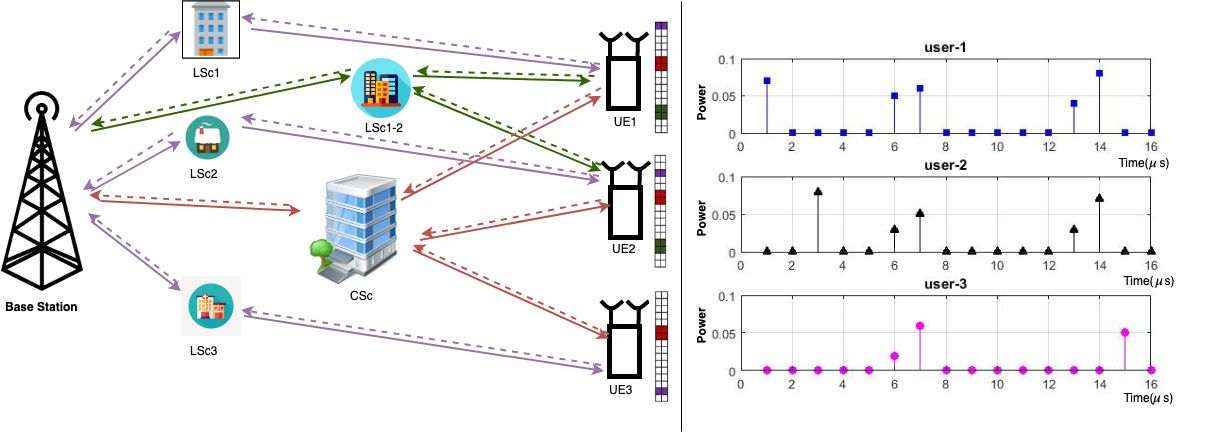
\includegraphics[scale=0.37]{figures/fig_ch_rec/joint_channelplus_cir.jpg}
\caption{System description of downlink (solid) and feedback link (dotted) for joint channel sparsity with local scatters (LSc) and common scatters (CSc), Channel impulse response is also given for all three users.}
\label{sys_fig}
\end{figure*}
Where $\mathbf{\beta}_l$ is the complex amplitude for $l^{th}$ path, $\tau_l$ is the  $l^{th}$  path delay, $\theta_{r,l}$ and $\theta_{t,l}$ are the transmitted and received path angles and $\mathbf{a}_r$, $\mathbf{a}_t$ represents array steering and response vectors of transmitted/received signal in the direction of $\theta_t$/$\theta_r$. To mitigate frequency selective fading the OFDM scheme is used \cite{reviwsparse,CRRM2011,Vizziello2013}. An OFDM symbol duration $T_{sym}=(N_o+G)\cdot T_s$ is considered, where $N_o$ is the number of subcarriers equally spaced in frequency at ${\Delta} f=\dfrac{1}{T_s}$, with the sampling time $T_s$, and $G$ is the guard interval in number of samples, which is set larger than the expected channel delay spread to further reduce the inter-symbol interference (ISI) \cite{reviwsparse}. 
\label{formulation}
\subsection{Distributed Joint Channel Sparsity Model}
\label{lbDis_JCS}
In any particular cell, there are some dominant scattering clusters whose position is determined from the specific attributes of the cell itself, like the presence of buildings or other propagation obstacles. These scatters can be shared by users regardless of their position \cite{Dict_learning}.  Massive MIMO experiments \cite{exp-vitual} prove that channel matrices at the user side is sparse due to the limited local scatters at the BS \cite{mimo-common-sparsity}, and maybe jointly correlated
due to the shared common local scattering clusters \cite{corr_pathdelay}. Thus, both per-link and joint channel sparsity can be exploited through CS-based solutions to reduce training and feedback overheads.
The inter-user channel sparsity can be further explained based on how scatters are shared among users: 
\begin{itemize}
  \item The scatters shared among all users are known as common scatters (CSc), for example, in Fig. \ref{sys_fig} CSc are shared among all UE, these common scatters will produce \textit{joint sparsity}.
  \item The scatters for a single user or shared among the subgroup of users is known as local scatters (LSc). For example, in Fig. \ref{sys_fig} LSc1, LSc2, and LSc3 are local scatters for UE1, UE2, and UE3 respectively, while, LSc1 and LSc2 are shared among UE1 and UE2. In the case of LSc, the inter-user joint sparsity will be limited to a sub-group of users sharing the LSc, this is termed as \textit{partial joint sparsity}. 
\end{itemize}

The presented research work considers a uniform linear array (ULA) model for both BS and user side antennas. To represent spatio correlation channel for ULA in angular domain, the virtual channel representation can be considered. The experimental studies in \cite{exp-vitual} confirms that spatial channel can be transformed into angular domain as follows:

\begin{equation}
\mathbf{H}_i^a=\mathbf{F}_{R_i}^H \mathbf{{H}}_i \mathbf{F}_{T_i} \text{,}\quad \quad \mathbf{H}_i=\mathbf{F}_{R_i} \mathbf{{H}}_i^a \mathbf{F}_{T_i}^H
\label{eq-VCM}
\end{equation}

 Where $\mathbf{F}_{R_i}\in \mathbb{C}^{N_r\times N_r}$ and $\mathbf{F}_{T_i}\in \mathbb{C}^{N_t\times N_t}$ represent the unitary  matrices with Fourier basis. This transforms the channel at BS and user side from a spatial domain to the virtual angle domain.
$\mathbf{H}_i^a \in \mathbb{C}^{N_r\times N_t}$ is the virtual channel representation and can be considered equivalent to the actual spatial channel $\mathbf{{H}}_i$ in Fourier domain \cite{exp-vitual}. The non-zero $(c,d)$-th entry of $\mathbf{{H}}_i^a $ indicates the spatial path from the $c$-th BS transmit direction to $d$-th receive direction of the $i^{th}$ user.
 Equation (\ref{eq-VCM}) has been used to represent the spatial channel in the angular domain with the sparsifying matrix F  \cite{mainref-joint,Dict_learning}. Although with angular domain representation channel sparsity is guaranteed, however, to obtain it explicitly for per link and joint channel sparsity, the design of sparsifying matrix $\mathbf{F}$ is very critical. In \cite{mainref-joint} and \cite{mainref-1bit} a sparsifying matrix $\mathbf{F}$ is considered as square DFT matrix, but in \cite{Dict_learning} and \cite{ourwork} it has been shown that by introducing more redundancy in sparsifying matrix $\mathbf{F}$ improved channel representation can be achieved, further details are discussed in section \ref{sec:dict_formation}.  
Fig. \ref{sys_fig} shows the system description with local and common scatters in a multi-user MIMO system. The left-hand side of the figure explains the joint sparsity structure by displaying varying support indexes (non-zeros entries) in different colors in the channel matrix. For example, the scatters shared among all users are represented by the common support $\Theta_c$ indicated in red, the support of the scatter shared only by some users is shown in green, and of the local scatters is represented in blue. The individual support $\Theta_i$ represents the non-zeros entries of each user. The left-hand side shows the position of the support, while the right-hand side shows that there will be different values for these supports. Besides, the right-hand side also gives a snapshot of the channel delay profile for different users in this hypothetically generated propagation environment.

The sparsity of the massive MIMO channel may be explained as follows \cite{mainref-joint,mainref-1bit,book_enrico}: 

\begin{enumerate}
\item \textbf{Intra-User Joint Sparsity (Individual joint Sparsity):}\\
Since there are more than one receiver antennas $N_r$  per user, the channel will exhibit intra-user joint sparsity. This effectively means that there will be channel dependency among different antennas of each user at the same time. This dependency is produced by local scatters.  Consequently, the receiver channel matrix elements will be extremely correlated and its row vectors will usually have the same sparsity support. Specifically, the matrix $\mathbf{H}_i^a$ is a row sparse and for each user $i$, the $j^{th}$ row vector $\mathbf{H}_i^a(j)$ will have same support $\Theta_i$ such that $0<|\Theta_i|\ll N_t$, i.e.,
\begin{equation}
    \Theta_{i1}=\Theta_{i2}=\hdots =\Theta_{iN_r}
    \simeq\Theta_i
\end{equation}
\item \textbf{Inter-User Sparsity (Distributed Joint Sparsity):}
Inter-user sparsity exploits the channel dependency among different users at the same time\cite{book_enrico}. It refers to the scenario of a massive MIMO system where different users are close enough to share some common scatter. Therefore, the channel matrices of different users will be highly correlated and will have common sparsity support $\Theta_c$:
\begin{equation}
    \Theta_c= \bigcap_{i=1}^{K} \Theta_i
\end{equation}

This common sparse support will be a subset of individual sparse support if users are sharing some common scatters, such that $\Theta_c \subseteq \Theta_i$. However, if there are only common scatters among users, then the individual sparsity support will be equal to the common sparsity support.
There is the possibility that none of the users are sharing any common scatter, in that case, $\Theta_c=\emptyset$  \cite{mainref-joint}.
\end{enumerate}

\subsection {\textbf{Limited feedback based channel recovery and beamforming}}
\label{LF_framework} 
\begin{figure*}[h!]
    \centering
    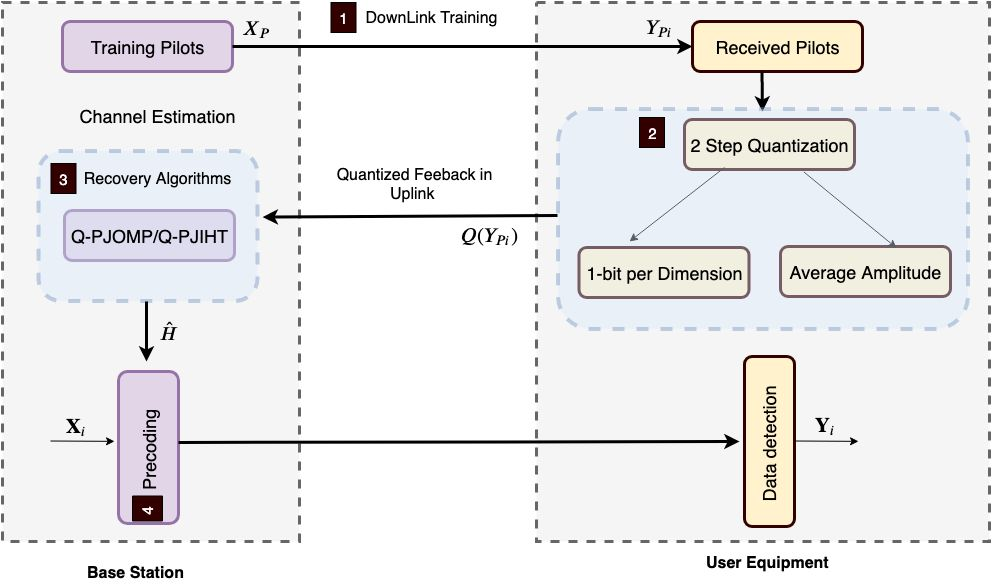
\includegraphics[scale=0.44]{figures/fig_ch_rec/flow_chart_MIMO.jpg}
   \caption{Flow chart of the complete procedure of CSI acquisition and utilization. }
    \label{fig:CSI_flow}
\end{figure*}

The current section discusses the overall procedure for channel recovery from the quantized feedback pilots and utilization of that estimate for transmit beamforming as shown in Fig. \ref{fig:CSI_flow}. The BS sends pilots in the DL, which are quantized at each UE and are fed back to BS via a dedicated uplink signaling channel. The BS utilizes these quantized pilots to exploit channel's hidden joint sparsity for channel estimation using distributed CS algorithms. Eventually, the recovered channel is employed for beamforming at the transmitter for more reliable data detection at the receiver. Each step is further explained as follows:  

 
$\bigstar$ \textbf{Step-1 Downlink training:}  
As discussed in Sec. \ref{sec:intro}, to obtain CSI of the DL at the transmitter in FDD, the pilots are sent in DL. For this purpose, the BS broadcasts $T$ common training symbols to the $K$ users over the downlink. Therefore, the received pilots for the $i^{th}$ user can be written as:
\begin{equation}
\mathbf{Y}_{pi} = \mathbf{H}_i \mathbf{X}_p + \mathbf{N}_i
\label{eq_channel_pilot}
\end{equation}
Where $\mathbf{X}_p  \in \mathbb{C}^{N_t \times T}$ is the concatenated transmitted pilots, and $\mathbf{Y}_{pi} \in \mathbb{C}^{N_r \times T}$ is the received pilots on each $i^{th}$ user as shown in step-1 of Fig. \ref{fig:CSI_flow}. \\
   
   
$\bigstar$ \textbf{Step-2 Quantization:}
The received pilots $\mathbf{Y}_{pi}$ are quantized at each UE to reduce the number of feedback bits, as shown in step-2 of Fig. \ref{fig:CSI_flow}. It is represented as $Q(\mathbf{Y}_{pi}$), however, the quantization process may also induces some error as follows: 
\begin{equation}
\mathbf{\hat{Y}}_{pi} =Q(\mathbf{Y}_{pi})+ \mathbf{\Gamma}_i
 = Q(\mathbf{H}_i \mathbf{X}_p + \mathbf{N}_i) + \mathbf{\Gamma}_i
\label{eq_qunatization}
\end{equation}
Where Q(.) is the uniform quantization function that maps the complex pilots to bits [+1, -1] and $\mathbf{\Gamma}_i$ is the quantization error. In the presented work, pilots are quantized by preserving both direction and amplitude, as opposed to \cite{mainref-1bit}, where pilots are quantized to the extreme 1-bit case. The 1-bit scheme lacks power information, having only directional information, this results in poor channel estimate. Therefore, we have considered averaged quantized amplitudes of the received pilot for each user. The averaged amplitude  $\mu_i=\frac{1}{P_t} \sum_i^{P_t} |\mathbf{Y}_{pi}|$ of the received complex pilot $\mathbf{Y}_{pi}$ is determined for each user.  Subsequently, these averaged amplitudes are quantized to 2 bits per user.  Furthermore, the direction information is  computed using 1 bit per dimension from the received pilots, given as:

\begin{equation}
\mathbf{Y}_{pi}=\text{sign(Re}(\mathbf{Y}_{pi}))+j\text{sign(Im}(\mathbf{Y}_{pi})) 
\label{eq_qunatization}
\end{equation}

The amplitude information $\mu$ is fed back along with the direction information to the BS,  this is further described in algorithm \ref{algo1}. \\
  
 
$\bigstar$ \textbf{Step-3 Channel recovery using CS:}
The quantized pilots determined in step 2 are fed back to BS in UL. At the BS, CS-based algorithms are applied to recover the channel. The BS employs the 2-bit partial amplitude information per users along with 1 bit per dimension direction information of each user to recover the channel jointly for all users. It is important to mention that as the users are sharing the channel, therefore, partial amplitude along with direction information is sufficient to jointly estimate the partially correlated channel. For this purpose, the CS-based JOMP \cite{mainref-joint} and BIHT algorithms \cite{mainref-1bit} are modified. This facilitates channel recovery using quantized feedback information.  We have proposed two novel distributed CS-based greedy algorithms for better analysis in terms of complexity and performance, The Q-PJIHT  \ref{algo2} and Q-PJOMP are given in algorithm \ref{algo3}, respectively. 

Further details of CS-based channel recovery and proposed CS algorithm is provided in section \ref{sec:dict_formation}. \\

$\bigstar$ \textbf{Step-4 Beamforming:}
During step 3 estimate of the channel, $\mathbf{\hat{H}}_i$  becomes available at the BS side, it is employed to achieve transmit beamforming, as shown in step 4 of Fig. \ref{fig:CSI_flow}. The precoding matrix is constructed by applying this estimate, it overcomes the inter-user interference and decorrelates users in a highly correlated environment. Furthermore, the precoding matrix is beneficial for data detection to decorrelate users. In particular, we have focused on minimum mean square error (MMSE) or regularized zero-forcing (RZF), as shown in equation (\ref{eqMMSE}). It attempts to maintain strong signal gain while limiting interference among users.  MMSE based precoding is more reliable than ZF, since ZF amplifies the noise in the presence of highly correlated user channel. Moreover, MMSE precoder is not only robust for MU-MIMO systems where users are located in the vicinity, but it also provides stable performance at high SNRs\cite{precding_survay}.  MMSE precoder is considered as the more suitable choice for linear precoding in MIMO based wireless systems \cite{precding_survay,precoding_emil}. For MMSE based precoding, the received signal model in equation (\ref{eq_channel}) is revisited  by including the beamforming matrix $\mathbf{W}$  as follows: 
\begin{equation}
\text{MMSE}
\begin{cases}
%\mathbf{{Y}}_{pi}=Q(\mathbf{Y}_{pi})\\
\mathbf{G}= \mathbf{\hat{H}}^H (\mathbf{\hat{H}} \mathbf{\hat{H}}^H +\lambda \mathbf{I} )^{-1 } \\
\eta= \sqrt{\frac{N_t}{Tr (\mathbf{G} \mathbf{ G}^H)}}\\
\mathbf{W}= \eta \mathbf{G} \\
\mathbf{Y}_i=\mathbf{X}_i \mathbf{W}_i \mathbf{H}_i +\mathbf{N}_i\\
%\mathbf{Y}_{pi}=Q(\mathbf{X}_p \mathbf{W}_i \mathbf{H}_i +\mathbf{N}_i) 
\end{cases}
\label{eqMMSE}
\end{equation}
 In the above equation, $\lambda= N_t \sigma^2 /K$ is the regularization factor, if $\lambda=0$, the MMSE precoder becomes equal to a ZF. The MMSE optimal precoder $\mathbf{G}$ is obtained from the estimated channel $\mathbf{\Hat{H}}$ of all users.
In the next step $\mathbf{G}$ is scaled with the power scaling factor $\eta$ to minimize the mean square error (MSE) under the  BS transmit power constraints \cite{power_MMSE}. Primarily, $\eta $ is used for power allocation at the BS to minimize the total power consumption under some given noise and interference related constraints. While $\lambda$ attempts to maintain the strong signal gain with limited interference among users.
Besides the MMSE precoder in equation (\ref{eqMMSE}), for comparison purpose an SVD based beamforming is also applied, as shown in equation (\ref{eqsvd}) . It can be noted that we do not assume perfect channel knowledge. Accordingly, the estimate of realistic channel can be decomposed using SVD, and is given as follows:  
\begin{equation}
 \mathbf{\hat{H}}_i=\mathbf{\hat{U}}_i \mathbf{\hat{\Lambda}}_i \mathbf{\hat{V}}_i^H
\label{eq-svd}
\end{equation}
Where $\mathbf{\hat{U}}_i\in \mathbb{C}^{N_r\times N_r}$ and $\mathbf{\hat{V}}_i\in \mathbb{C}^{N_t\times N_t}$ represent the unitary  matrices, such that $\mathbf{\hat{V}}_i^H\mathbf{\hat{V}}_i=\mathbf{\hat{U}}_i\mathbf{\hat{U}}_i^H = \mathbf{I}$ and
$\mathbf{\hat{\Lambda}}_i\in \mathbb{C}^{N_r\times N_t}$ is a diagonal matrix. But, as we have considered realistic channel $\mathbf{\hat{H}}_i$,  therefore, the estimated channel characteristics will not exactly match with that of the ideal channel. Consequently, the unitary property $\mathbf{{V}}_i^H\mathbf{\hat{V}}_i = \mathbf{I}$ does not hold any more and this may induce interference.  Nevertheless, these ramifications can be combatted provided the channel estimate is robust. Based on SVD decomposition, the equation (\ref{eq_channel}) is revised and beamforming equations can be given as: 
\begin{equation}
\text{SVD}
\begin{cases}
\mathbf{\hat{X}}_i= \mathbf{\hat{V}}_i^H  \mathbf{X}_i    \\
\mathbf{{Y}}_i=\mathbf{H}_i \mathbf{X}_i+\mathbf{N}_i=(\mathbf{U}_i \mathbf{\Lambda}_i \mathbf{V}_i^H)  \mathbf{X}_i+\mathbf{N}_i , \,\,\,\,\,\,\,\,\,\, \forall_i \in K\\
\mathbf{\hat{U}}_i^H\mathbf{{Y}}_i=\mathbf{\hat{U}}_i^H (\mathbf{U}_i \mathbf{\Lambda}_i \mathbf{V}_i^H)   \mathbf{\hat{V}}_i \mathbf{\hat{X}}_i+\mathbf{\hat{U}}_i^H\mathbf{N}_i, \,\,\,\,\,\,\,\,\,\, \forall_i \in K\\
\mathbf{\hat{Y}}_i= \mathbf{\Lambda}_i \mathbf{\hat{X}}_i+\mathbf{\hat{N}}_i
\end{cases}
\label{eqsvd}
\end{equation}
Where $\mathbf{\hat{X}}_i$ is the precoded signal at the transmitter, $\mathbf{\hat{N}}_i= \mathbf{\hat{U}}_i^H\mathbf{N}_i$ is the noise term, and $\mathbf{\hat{Y}}_i =\mathbf{\hat{U}}_i^H\mathbf{{Y}}_i$ is the decoder for the transmit beamformer at the receiver side. 

\begin{algorithm}[H]
\SetAlgoLined
 \textbf{Step-1:} A common training pilot vector $\mathbf{X}_p$ is transmitted from BS to all the users.\\ 
 \textbf{Step-2:} Each user's received pilots are quantized using two steps:
 \begin{enumerate}
     \item[(a)]  The averaged amplitude $\mu_i$ of the received  pilot vector $\mathbf{Y}_{pi}$ is calculated for each user. Then these averaged amplitudes are quantized to 2 bits per user;
     \item[(b)] the sign information is achieved with 1 bit per dimension from the received pilots:\\ $S(\mathbf{Y}_{pi})=S(\mathbf{H}_i\mathbf{X}_{p}) $ such that\\ $S(\mathbf{Y}_{pi})=\text{sign(Re}(\mathbf{Y}_{pi}))+j\text{sign(Im}(\mathbf{Y}_{pi}))$ .
 \end{enumerate}
 \textbf{Step-3:} Each user feedbacks the obtained quantized and reduced $\mathbf{Y_{pi}}$  to BS.\\
\textbf{Step-4:} The channel is jointly recovered for all users from the quantized feedback pilots $\mathbf{Y}_{pi}$ using distributed CS at BS.\\
\caption{Joint channel recovery framework from quantized feedback}
 \label{algo1}
\end{algorithm}
 
\section{Compressive Channel estimation with limited feedback}
\label{sec:dict_formation}
In sec. \ref{LF_framework}, the overall framework has been described, it consists of channel estimation, beamforming matrix design, and data detection. The channel estimation is performed at the BS side using the quantized pilots received on UL from UE, as indicated in step-3 of Fig. \ref{fig:CSI_flow}.  The current section will discuss compressed sensing algorithms and dictionary design in more detail. 

\subsection{Comparison of dictionary and DFT basis for measurement matrix design}
A channel that exhibits only a few dominant propagation paths may be considered sparse and is approximated as a linear combination over a known basis or dictionary, resulting in a sparse channel response \cite{reviwsparse}.  Conventionally, DFT basis $\phi$ have been utilized for sparse channel representation \cite{reviwsparse,beamblock,dft,mainref-joint,mainref-1bit} as shown below.  
    \[
 \mathbf{    \phi= \frac{1}{\sqrt{N_t}}
    \begin{bmatrix}
e^{-j2\pi k_{1,1}} &\dots& e^{-j2\pi k_{1,N_t}} \\
e^{-j2\pi k_{2,1}} &\dots& e^{-j2\pi k_{2,N_t}} \\
\vdots & \ddots & \\                                          
e^{-j2\pi k_{N_t,1}}  &\dots& e^{-j2\pi k_{N_t,N_t}} \\
    \end{bmatrix}}
    \]    \\
The usage of the DFT basis is compliant with the theoretical results of signal estimation in CS\cite{Candes08}, therefore, the DFT basis are employed in sparse channel representation. Considering normalized DFT basis $\phi$ as a sparsifying matrix, the sparse channel response can be written as, $\mathbf{\hat{H}}_i=\phi \mathbf{B}_{si}$, where $\mathbf{B}_{si} \in \mathbf{C}^{N_t \times N_r}$ is the sparse matrix. As described earlier in equation (\ref{eq-VCM}), such modeling is applied to represent spatial channel response into the angular domain, also known as the virtual channel model. Though, the DFT basis represents the channel only in a few directions. In a real-world scenario, the actual signal can emanate from arbitrary directions, which may differ from the one represented in the DFT matrix. This results in leakage effect and poor channel estimate.  In case the channel is highly correlated or exhibits multipath, the leakage effect worsens even further \cite{Dict_learning}. 

To estimate the channel accurately, a robust and effective basis is an essential prerequisite. To construct an improved and substantial basis or dictionary, we extended the squared DFT matrix by proposing added redundancy and considering the channel delay profile as in \cite{ourwork}. The objective is to build a more flexible and enhanced representation of the channel. In the dictionary formulation, the channel delay profile $\tau_{ch}$ can be represented using OFDM sample time $T_s$ and guard interval $G$, for each dictionary point as follows:
    \begin{equation}
\mathbf{    
\tau}_{ch}=[0,\alpha,2\alpha,\cdots \cdots (M-1)\alpha]
    \end{equation}  
 Where M is the length of dictionary column, $\alpha$ is step size in the range of $0$ to $M$ and is given as $\alpha=[G\cdot T_s-(G\cdot T_s/M$)]. To avoid inter-symbol interference (ISI), the step size $\alpha$ is constrained with $\tau_\text{max}$  not exceeding $G$, i.e., ($\tau_\text{max}< G$)\cite{reviwsparse}.
\textcolor{black}{To formulate the dictionary basis $\mathbf{D}$ for the channel response, the OFDM symbol duration $T_\text{sym}$ and the delay profile can be utilized as follows:}\\
\[
\mathbf{    D=
    \begin{bmatrix}
    e^{-j2\pi k_1 \tau_1} & e^{-j2\pi k_1 \tau_2}&\cdots& e^{-j2\pi k_1 \tau_M} \\
    e^{-j2\pi k_2 \tau_1} & e^{-j2\pi k_2 \tau_2}&\cdots& e^{-j2\pi k_2 \tau_M} \\
    \vdots & \dots & \\                                        
    e^{-j2\pi k_{N_t}\tau_1} & e^{-j2\pi k_{N_t}\tau_2} &\cdots& e^{-j2\pi k_{N_t}\tau_M} \\
    \end{bmatrix}
    }    \]
Where $\tau(m)=  \tau_\text{ch}(m)/T_\text{sym}$ is the channel delay normalized by OFDM symbol duration $T_\text{sym}$, having $m=\{1,2,\cdots M\}$. 
To effectively estimate a channel with multiple paths, the guard interval and channel delay profiles must be taken into account.
Comparable to DFT basis, the channel response can be sparsely represented in dictionary $\mathbf{D}$ based sparsifying matrix, $\mathbf{\hat{H}}_i=\mathbf{D} \mathbf{B}_{si}$. The $\mathbf{B}_{si}  \in \mathbf{C}^{M \times N_r}$ is the sparse matrix such that ($\|\mathbf{B}_{si} \|_0 \ll N_t$). The equation \ref{eq_channel} can be rewritten as:
\begin{equation}
    \mathbf{Y}_{pi}= \mathbf{A} \mathbf{\hat{H}}_i + \mathbf{N}_i= \mathbf{A} \mathbf{D} \mathbf{B}_{si}  +\mathbf{N}_i
    \label{eq-cs_model}
\end{equation}
Where $\mathbf{A}$ is the measurement matrix, it can be constructed utilizing the transmitted pilots $\mathbf{X}_p$  and sub DFT basis or sub-dictionary. In further detail, a sub-dictionary $\mathcal{D} \in \mathbf{C}^{P_t \times N_t}$ can be derived from dictionary $ \mathbf{D} \in \mathbf{C}^{N_t \times M}$,  subsequently, the measurement matrix $\mathbf{A}$ can be expressed as:
\begin{equation}
 \mathbf{A}_\mathcal{D}= \mathbf{X}_p^H \otimes \mathbf{\mathcal{D}}  
    \label{eq-Ad}
\end{equation}
The basis $\mathcal{D}$ comprises of specially selected rows of $\mathbf{D}$  associated with the pilot locations \cite{reviwsparse}, as shown in equation (\ref{mat_dic}). 
 The transmitted pilots $\mathbf{X}_p$ are built according to a Rademacher distribution (RD) consisting of equally likely symbols taken from $[+1,-1]$.  Subsequently, they are multiplied by a phase rotation and can be formulated as $\mathbf{X}_{P_n}=[ P_1e^{-j\pi l_1}  P_2e^{-j\pi l_2}  \hdots   P_te^{-j\pi l_{P_t}}]$, where $P_t$ represents the total number of transmitted pilots for the $n^{th}$ transmit antenna.
     \begin{align}
    \label{mat_dic}
    \mathbf{A}_{\mathcal{D}} &=  \mathbf{X}_p^H \otimes
    \begin{matrix}
    \begin{bmatrix}
    e^{-j2\pi k_1 \tau_1}\cdots e^{-j2\pi\cdot k_1\tau_{N_t}} \\
    e^{-j2\pi k_2\tau_1}\cdots e^{-j2\pi\cdot k_2\tau_{N_t}} \\
    \vdots  \\    
    e^{-j2\pi k_{P_t} \tau_1} \cdots e^{-j2\pi \cdot k_{P_t}\tau_{N_t}} \\
    \end{bmatrix} 
    \end{matrix}
    \end{align}
Where $\mathbf{A}_{\mathcal{D}} \in \mathbf{C}^{P_t \times N_t}$ represents  the measurement matrix constructed from known pilots and dictionary.
For comparison, the measurement matrix $\mathbf{A}$ is computed using two equivalent approaches; firstly, starting from $\mathbf{D}$ as already discussed in equation (\ref{mat_dic}), and secondly, through DFT basis \textbf{$\phi$}, that is shown in equation (\ref{mat_dft}). 
\begin{align}
     \mathbf{A}_\phi &= \mathbf{X}_p^H \otimes
     \begin{matrix}
     \label{mat_dft}
     \begin{bmatrix}
     e^{-j2\pi k_{1,1}} &\dots& e^{-j2\pi k_{1,N_t}} \\
     e^{-j2\pi k_{2,1}} &\dots& e^{-j2\pi k_{2,N_t}} \\
     \vdots & \ddots & \\                              
     e^{-j2\pi k_{{P_t},1}}  &\dots& e^{-j2\pi k_{{P_t},N_t}} \\
     \end{bmatrix}
     \end{matrix}
\end{align}
The $\mathbf{A}_{\phi} \in \mathbf{C}^{P_t \times N_t}$ is calculated  from DFT sub matrix. It is noteworthy that the construction of the measurement matrix $\mathbf{A}_{\mathcal{D}}$  is different from $\mathbf{A}_{\phi}$ used by \cite{mainref-joint,mainref-1bit}.\\
In the case $\mathbf{D}$, $\mathbf{A}$ and $\mathbf{Y}_{pi}$ are known in equation (\ref{eq-cs_model}),  the solution of $\|\mathbf{B}_{si}\|_0$  will yield the channel estimate. Although, solving $\|\mathbf{B}_{si}\|_0$ will provide an exact solution, however, it is NP-hard problem. The severity of predicament can be reduced if we relax $l_0$  to $l_1$ or $l_2$ norm such that min$\|\mathbf{B}_{si}\|_{1,2}$.
The aforementioned optimization problem can be formulated
for joint channel estimation at BS \cite{Alesii2015}, as shown in equation (\ref{mini-problem}).
 \begin{equation}
      \underset{\{\mathbf{B}_{si} \forall_i \}}{\text{min} } \sum_{i=1}^K \|\mathbf{Y}_{pi} -\mathbf{A} \mathbf{D} \mathbf{B}_{si}  \|_2 \le \epsilon
     \label{mini-problem}
\end{equation}
However, the above mentioned minimization problem is very challenging, because of both individual and joint sparsity among different users.
By solving the above optimization problem, instead of obtaining a channel estimate with training overhead proportional to $N_t$, it is possible to obtain a good channel estimate which is proportional to the sparsity level $s$ of the sparse channel such that $s \ll N_t$.
\subsection{Constraints for Stable Recovery}
Several constraints and properties have been discussed in the literature for the stable sparse signal reconstruction for measurement matrix $\mathbf{A}$. For example, the accuracy of recovery parameters can be determined in a case $\mathbf{A}$ satisfies the null space property (NSP), restricted isometry property (RIP) or mutual coherence. However, null space property (NSP) or restricted isometry property (RIP) are difficult to measure.  Although,  for guaranteed sparse signal recovery,  it is adequate to only satisfy the mutual coherence property for the measurement matrix $\mathbf{A}$  \cite{RIP_Mutual}\cite{reviwsparse}. \\
\textit{Theorem 1 :} In mutual coherence the maximum absolute and normalized inner
product between the columns of measurement matrix $\mathbf{A}$ is analyzed.
It determines the correlation among the columns of the measurement matrix and can be formulated as \cite{reviwsparse}: 
\begin{align}
    \mu\{\mathbf{A}\}= \underset{1\le i \le j \le N_t, i\neq j}{\text{max} }\frac{|\mathbf{A}_i, \mathbf{A}_j|}{\| \mathbf{A}_i\|_2 \| \mathbf{A}_j\|_2} \nonumber \\
    =\underset{1\le i \le j \le N_t, i\neq j}{\text{max} }\frac{|\mathbf{A}_i^H \mathbf{A}_j|}{\| \mathbf{A}_i\|_2 \| \mathbf{A}_j\|_2}
\end{align}
The mutual coherence of $\mathbf{A}$ at the pilot locations can be written as:
\begin{align}
\mu\{A\}&=\underset{1\le i \le j \le N_t, i\neq j}{\text{max}}\\
& \frac{\sum^{P_t}_{l=1} (\mathbf{X}_p(k_l)  e^{-j2\pi k_l \tau_i/N_t}) (\mathbf{X}_p(k_l)  e^{j2\pi k_l \tau_j/N_t})}{\sum^{P_t}_{l=1}|\mathbf{X}_{pl} |^2} \nonumber \\
&=\underset{1\le i \le j \le N_t, i\neq j}{\text{max}} \frac{\sum^{P_t}_{l=1} |\mathbf{X}_p(k_l)|^2  e^{j2\pi k_l \tau (j-i)/N_t}) }{\sum^{P_t}_{l=1}|\mathbf{X}_p(k_l) |^2}       
\label{eq-mutual_coh}
\end{align}
Since our complex pilots are equi-power, therefore, we can conveniently assume that:
($|(\mathbf{X}_p(k_1) |= |(\mathbf{X}_p(k_2) | ..... =|(\mathbf{X}_p(k_{P_t})|=1$). 
Consequently, the normalized equation (\ref{eq-mutual_coh}) can be re-written as:
\begin{align}
\mu\{\mathbf{A}\}=\underset{1. \le i \le j \le N_t, i\neq j}{\text{max}} \sum^{P_t}_{l=1} \frac{1}{P_t} 1 e^{j2\pi k_l \tau_(j-i)/N_t}) \label{eq-mutual_coh_final}
\end{align}
From equation (\ref{eq-mutual_coh_final}) it is evident that the value of $\mu\{\mathbf{A}\}$ will not rely on the pilot symbols, instead it only depends on the columns of dictionary  $\mathbf{D}$ selected. 
The dictionary $\mathbf{D}$  is a sparsifying matrix and is employed to realize the channel, it is mostly designed a prior channel estimation. Consequently, during the channel estimation, if $\mathbf{D}$  is constructed tactfully, $\mu\{\mathbf{A}\}$ will remain small and fixed. In short, from theorem 1 it is obvious that for efficient channel estimation minimum coherence value is desired, therefore, our objective is to minimize $\mu\{\mathbf{A}\}$. The value of $\mu$ is generally in the range of 0-1, as for better recovery the smaller value is desired \cite{RIP_Mutual}.\\
The sparse channel reconstruction is based on the assumption that the channel response is sparse. In other words, the channel energy is uniformly distributed among the few dominant taps. However, the exact positions of these dominant taps are not known a priori and must be estimated for the effective channel measurement \cite{diclng}. To estimate exact positions, a redundant basis $\mathbf{D}$ is required. 
In conclusion, from the reduced and quantized pilots $\mathbf{Y}_{pi}$ and the dictionary $\mathbf{D}$ the channel estimate $\mathbf{\hat{H}}_i$ is obtained at BS by utilizing the CS algorithms (i. e., Q-PJOMP, and Q-PJIHT), discussed in detail in the following subsection.

\subsection{ Algorithm formation for Sparse Channel Estimation}
In some cases, it has been observed that the sparse data exhibit special structure in its measurement, for example, in a certain measurement, the sparse coefficients may form a group or block of zero and non zero entries. Such sparsity structure is known as group/block sparsity \cite{beamblock,our_intrabody,Dekorsy12}. This sparsity structure can be formulated by employing multiple measurements, known as joint sparsity \cite{mainref-joint,mainref-1bit,antenna_spacing_sparse}. In joint sparsity, each row of N vectors tends to be zero or non-zero simultaneously. The research work \cite{structured_sparsity} demonstrates that the performance gain can be achieved if such structures are exploited in sparse measurements of the observed data. 
Consequently,  the hidden joint sparsity structure of the correlated multi-users MIMO channel is exploited, based on this hidden sparsity the DCS algorithms Q-PJOMP and Q-PJIHT  are proposed. In both methods, it has been assumed that the sparsity information is known at the BS. This can be determined at the BS using slow-timescale stochastic learning \cite{stochastic_ch_info,scattering_model}.
The proposed Q-PJOMP and Q-PJIHT are presented in algorithm \ref{algo2} and \ref{algo3} respectively. In algorithm \ref{algo2} and \ref{algo3},  2-step quantization methods are labeled as $A$, 1-bit binary algorithm is indicated with $B$ and the common lines to both algorithms are marked with $AB$. If the algorithm \ref{algo2} and \ref{algo3} are viewed without label $A$ they transform into 1-bit Q-PJOMP/Q-PJIHT.  Similarly, inspecting the algorithms without label $B$ will convert them into the 2-step Q-PJOMP/Q-PJIHT. Both of the algorithms are presented subsequently in the following subsections.

 \subsubsection{  \textcolor{black}{Channel Recovery with Q-PJOMP}}
 The current subsection describes Q-PJOMP for partially joint channel estimation. Although, several research works present the solution with joint sparsity through OMP based approaches \cite{CIR_timevaring,somp}, however, the system with individual and partially joint sparsity still requires additional investigation.
{\begin{center}
\scalebox{0.8}{
\begin{minipage}{1.2\linewidth}
\begin{algorithm}[H]
\SetAlgoLined
\begin{enumerate}
 \item[1 (AB):]\textbf{Input:}{$\{\mathbf{Y}_{pi}: i \in K\}$,  $\mathbf{D}$
\item[2 (AB):] Measurement matrix $\leftarrow \mathbf{A} \}$,
support $= s_c,s_i $
 \item[3 (A)\,\, :]Averaged  quantized amplitude $\leftarrow Q(\mathbf{\mu})$ 
\item[4 (AB):]$\{Thresholds: \eta_1<1 , \eta_2>1 \}$}
\item[5 (AB):]\textbf{Output:}{ Channel estimate $\mathbf{\hat{H}}_i$}\\
\rule{0pt}{4ex}    
%\input{Y_i: i \in K}, A,{\Theta_i: i \in K}
\textbf{Procedure:}\\
 \textbf{Step 1 - Initialization:}
 \item[6 (AB):]support :$\{\Theta_i=0 , \Theta_c=0 $\}
  \item[7 (A)\,\, :] $\mathbf{\mu'}\leftarrow Q'(\mathbf{\mu}$) 
\item[8 (AB):] Compute $\mathbf{Y}_{pi}$ from (\ref{eq_qunatization}) and $\mathbf{A}$ from (\ref{mat_dic}) or (\ref{mat_dft})
\item[9 (A)\,\, :]The angle of $\mathbf{Y}_{pi}$ and the de-quantized amplitude are used to rebuilt $\mathbf{Y}_{pi}$\\
 $ \mathbf{Y}_{pi} \leftarrow  \mathbf{\mu'} \Big(  cos\theta_{\mathbf{Y}_{pi}} + j  sin\theta_{\mathbf{Y}_{pi}} \Big)$
  and 
  \item[10 (AB):]Initialize residual $\mathbf{Res}_i=\mathbf{Y}_{pi}$ 
  \rule{0pt}{4ex}
 \item[11 (AB):]\textbf{Step 2 - Identify the common support: \\
 while $t\le s_c$ or $\| \mathbf{A}^H \mathbf{Res}_i \|_F^2 \ge \eta_1 $  then} \\ 
 identify the common support $\Theta_c $ that solves optimization problem \\
 \hspace*{\algorithmicindent} 
     $\Theta_t\leftarrow\underset{s} {Arg max} \sum_i^K |\langle \mathbf{A}_s^H \mathbf{Res}_i \rangle|$\\ \hspace*{\algorithmicindent}
      $\Theta_c \leftarrow \Theta_c \cup \Theta_t $  
\item[12 (AB):] Determine the orthogonal projector $\mathbf{P}_o$ onto the span of the atoms indexed in $\Theta_c$ \\              \hspace*{\algorithmicindent}   
     $\mathbf{P}_o \leftarrow (\mathbf{A}_s)(\mathbf{A}_s)^\dagger $\\
     \hspace*{\algorithmicindent} 
    $ \mathbf{y}_o \leftarrow \mathbf{P}_o \mathbf{Y}_{pi} $\\
%\item[13 B\,\, :]$\mathbf{y} \leftarrow sign(Re(\mathbf{y}_o)+jsign(Im(\mathbf{y}_o)$
Residual Update:
     %\hspace*{\algorithmicindent}
     \item[13 (B)\,\, :]$\mathbf{Res}_i \leftarrow\mathbf{Y}_{pi} -\text{sign(Re}(\mathbf{y}_o))+j\text{sign(Im}(\mathbf{y}_o))$
  \item[14  (A)\,\, :]  $ \mathbf{Res}_i \leftarrow \mathbf{Y}_{pi}- \mu' \Big(  \text{cos}\theta_{y_o} + j\text{sin}\theta_{y_o} \Big)$\\
    \hspace*{\algorithmicindent}
   $ t \leftarrow t+1 $ \\
 \textbf{end}
 \rule{0pt}{4ex}
 \item[15 (AB):]\textbf{Step 3 - Identify the individual support: initialize $\Theta_i \leftarrow \Theta_c $
 \\while $t_i \le |s_i-s_c|$ or $ \|\mathbf{Res}_i\|_F^2 \le \eta_2 $ then} \\ \hspace*{\algorithmicindent}
 $\Theta_{ti}\leftarrow\underset{s}{\text{Arg max}} |\langle \mathbf{A}_s^H \mathbf{Res}_i  \rangle|$\\ \hspace*{\algorithmicindent}
  $\Theta_i\leftarrow \Theta_i \cup \Theta_{ti} $\\
 Residual Update:
 \hspace*{\algorithmicindent}
  %\item[16  B\,\, :]   $\mathbf{y} \leftarrow sign(Re(\mathbf{y}_o)+jsign(Im(\mathbf{y}_o)$
     \hspace*{\algorithmicindent}
  \item[16  (B)\,\, :] $\mathbf{Res}_i \leftarrow \mathbf{Y}_{pi}-(\text{sign(Re}(\mathbf{y}_o))+j\text{sign(Im}(\mathbf{y}_o))$
 \item[17  (A)\,\, :]   $ \mathbf{Res}_i \leftarrow \mathbf{Y}_{pi}-\mathbf{\mu'} \Big( \text{cos}\theta_{y_o} + j\text{sin}\theta_{y_o} \Big)$\\
  \hspace*{\algorithmicindent}
   $ t_i \leftarrow t_i+1 $\\
   \textbf{end}\\
   \rule{0pt}{4ex}
\textbf{Step 4 - Channel estimate}
The channel estimate is obtained 
\item[18 (AB):]$\mathbf{B}_{si}=(\mathbf{A}_{\Theta_i})^{\dagger}\mathbf{Y}_{pi}$\\
$\mathbf{\hat{H}_i}=\mathbf{D B}_{si}$
\hspace*{\algorithmicindent} 
\end{enumerate}
 \caption{ Quantized Partially Joint-OMP}
 \label{algo2}
\end{algorithm}
\end{minipage}}\end{center}
}

 For example, \cite{somp} investigates simultaneous joint OMP (SOMP) for multiple measurements sharing joint support. 
 In the current work, the system with individual and partially joint support is considered. To handle this kind of structured sparsity, in the literature some works are already present. For example, in \cite{SD-omp} a generalized joint sparsity model (GJSM) is presented.  Another research work \cite{mainref-joint} applies GJSM to exploit the hidden joint sparsity in massive MIMO channels for efficient resource utilization. However, their main objective is to reduce the training overhead, which turns out in lowering the feedback overhead. However, the number of feedback bits is still very high. 
Therefore, our focus is not only to reduce the number of measurements by taking advantage of joint sparsity structure among users channel but also to limit the number of feedback bits through a 2-step quantization process, while ensuring efficient reconstruction. To reduce the training overhead, our approach is inspired by \cite{mainref-joint} and \cite{ourwork}. In \cite{mainref-joint} the training overhead is lowered by considering the partially joint support structure among the user's channel. While in our previous work \cite{ourwork} it is achieved by utilizing a flexible and robust dictionary-based measurement matrix.
Besides reducing the training overhead, our work also lowers the number of feedback bits by introducing a 2-step quantization method.  
Q-PJOMP is based on a greedy algorithm select-discard OMP (SD-OMP) \cite{SD-omp}. It can perform individual as well as partially joint sparse channel approximation by choosing the "best match" projection of multi-user quantized received pilots onto the span of the measurement matrix.
 Initially, the received pilots are recomputed applying the de-quantized mean vector $\mu$ and the angle of 1-bit quantized vector $\mathbf{Y}_{pi}$ (line 9 in algorithm \ref{algo2}).  Subsequently, the algorithm detects the common support for all the users, which consists of jointly selecting one column from the measurement matrix $\mathbf{A}$  in each iteration (line 11 step-2 in algorithm \ref{algo2}). The main intuition behind this selection is to determine an atom (column index) that contributes to the maximum amount of residual energy across all signals\cite{SOMP_energy}.  The indices that appear in common support $\Omega_c$ are likely to be estimated by most of the users. In each iteration, new support is appended to the existing support set unless a stopping criterion is satisfied. 
Another important step is to orthogonalize the residual $\mathbf{Res}_i$ with the selected atom (column) of the measurement matrix (line 12 of Algorithm 2) so that each atom is chosen only once as in \cite{omp,somp}.  In the next step, the individual support of each user is identified as in standard OMP  (lines 15 step-3 in algorithm \ref{algo2})  \cite{omp}. Indeed, besides the common support, also a few individual supports may be present in each signal. Note that the indices of the measurement matrix which were already been taken by common support, are discarded by the individual support. The rest of the procedure is the same as the common support identification.
Afterward, the complex pilot at each support index is recomputed and updated (lines 13 and 14 for common support and lines 16 and 17 for individual support in algorithm \ref{algo2}) in a design similar to  \cite{qomp}, although the overall procedure and problem are different from the proposed.
Finally, the channel is estimated using the LS approach (lines 18 step-4 in algorithm \ref{algo2}). 
To achieve stable recovery, there are different stopping criteria. For example, the algorithm will run for a particular number of iteration or will be executed until the norm of residual remains positive $\| \mathbf{Res}_i\| \ge \eta_2 $. In our case, the system will halt if the correlation between the atom of a matrix \textbf{A} and the residual drops below a threshold $\eta_1;$, which we set $(\eta_1= 0.04)$ in our simulation.
\subsubsection{Channel Recovery with Q-PJIHT}
For comparison purposes, Q-PJIHT is presented for partially joint channel estimation. In \cite{BIHT} 1-bit quantization is proposed, later to reduce hardware cost and system processing burden, the research work \cite{mainref-1bit} utilizes this 1-bit per dimension to estimate the partially joint channel in a massive MIMO system. 
The proposed Q-PJIHT algorithm explores both individual and  joint sparsity support as in \cite{mainref-1bit}, however, we apply a different quantization procedure, that includes the amplitude as well as the sign information. The purposed work also selects the optimal step size ($\eta$) depending on the sparsity level and dictionary length $ M$. Indeed, since IHT is a gradient descent based algorithm, its step size must be chosen optimally for better convergence \cite{Aiht}. Although standard IHT based algorithms are computationally simple and take less memory than standard OMP based methods.  For example, the computational complexity of the standard IHT is O(m n) while for the OMP is O(s m n). However, they have several challenges while dealing with the practical problem. As an example, the stable signal recovery highly depends on the selection of step size $\eta$ and sparsity parameter \cite{Aiht}.
 \section{PERFORMANCE EVALUATION} 
In the current section, the performance of the proposed scheme is evaluated using various CS techniques and different metrics. The proposed 2-step Q-PJIHT is compared with 1-bit Q-PJIHT whose algorithmic construction is inspired by 1-bit BIHT \cite{mainref-1bit}. The 2-step Q-PJIHT differs from 1-bit BIHT in terms of considering channel direction and partial amplitude information. Similarly, the Q-PJOMP is proposed and its 1-bit and 2-step versions are taken into account for analysis. Q-PJOMP has considered the equivalent joint channel sparsity model as in  JOMP \cite{mainref-joint}. Moreover, both Q-PJIHT and  Q-PJOMP differ from \cite{mainref-joint}, \cite{mainref-1bit} in terms of employing more robust sparsifying basis $\mathbf{D}$. The primary goal of this presented framework is to reduce the number of measurements and feedback bits while preserving high performance.  
\subsection{Simulation Setup}
We consider a MIMO-OFDM system, with $N_t=128$ transmit antennas, $N_r=2$ receive antenna and $K=10$ number of users. The BS uses $256$ OFDM subcarriers for downlink transmission while some sub-carriers are employed for pilot sequences and others for data. Specifically, during the first phase of training, only training pilots are sent without data, while in the second phase both data and pilots are transmitted in combo fashion. The dictionary length $M$ is set to $300$, whose value can be increased to reduce the error rate at the cost of higher processing. After varying $M$ up to $512$ we selected $300$ as a good compromise between performance and computation.
\begin{center}
\scalebox{0.8}{
\begin{minipage}{1.2\linewidth}
\begin{algorithm}[H]
\SetAlgoLined
\begin{enumerate}
\item [1 (AB):]\textbf{Input:}$\{\mathbf{Y}_{pi}: i \in K\}$ , $\mathbf{D}$
\item [2 (AB):]Measurement matrix $\leftarrow \mathbf{A} \}$
\item [3 (AB):]Sparsity level S $ \leftarrow s_c,s_i $,
\item [4 (A) : ] Averaged quantized amplitude $\leftarrow Q(\mathbf{\mu})$ 
\item [5 (AB):] Step size: $\eta \leftarrow \frac{1-\sqrt{\frac{S}{M}}}{M}$
\item [6 (AB):]\textbf{Output:} Channel estimate $\mathbf{\hat{H}}_i$ \\
\rule{0pt}{4ex}    
%\input{Y_i: i \in K}, A,{\Theta_i: i \in K}
\textbf{Procedure:}\\
 \textbf{Step 1 - Initialization:} 
\item [7 (A) : ]  $\mathbf{\mu}' \leftarrow Q'(\mathbf{\mu})$
\item [8 (AB):] Compute $\mathbf{Y}_{pi}$ from (\ref{eq_qunatization})  and $\mathbf{A}$ from (\ref{mat_dic}) or (\ref{mat_dft})
 \item [9 (AB):] The angle of $\mathbf{Y}_{pi}$ and the de-quantized amplitude are used to rebuilt $\mathbf{Y}_{pi}$
 \item [10 (A) : ] $ \mathbf{Y}_{pi} \leftarrow  \mu' \Big(  \text{cos}\theta_{\mathbf{Y}_{pi}} + j  \text{sin}\theta_{\mathbf{Y}_{pi}} \Big)$ 
\item [11 (AB):]  Initialize residual $\mathbf{Res}_i^o=\mathbf{Y}_{pi}$ \\
$\mathbf{B}_{si}^o \leftarrow \mathbf{A}^H  \mathbf{Res}_i^o$\\
 $\Theta_i\leftarrow 0$ \\
 %$\Theta_c^o\leftarrow supp ( A^H Res^0)$ \\
% $y^o \leftarrow  H_T(supp ( A^H Res^o ) ) $\\ 
$\Theta_c \leftarrow  0$\\
\rule{0pt}{4ex}    
\textbf{\textcolor{black}{Step 2 while( maximum iteration) do}}
\hspace*{\algorithmicindent} 
\item [12 (AB):]\hspace*{\algorithmicindent} $\mathbf{B}_{si}^{n+1}=\mathbf{B}_{si}^n+ \eta \mathbf{A}^H \mathbf{Res}_i^n $
 \hspace*{\algorithmicindent} 
\item [13 (AB):] Identify the common support $\Theta_c $ that solves the optimization problem \\\hspace*{\algorithmicindent} 
     $\Theta_t\leftarrow\underset{s}{\text{Arg max}} \sum_i^K |\langle \mathbf{A}_s^H \mathbf{Res}_i \rangle|$\\ \hspace*{\algorithmicindent}
      $\Theta_c \leftarrow \Theta_c \cup \Theta_t $\\
      Repeat the process $s_c$ times
\item [14 (AB):] Identify the individual support: Initialize $\Theta_i \leftarrow \Theta_c $\\
\hspace*{\algorithmicindent} $\Theta_{ti}\leftarrow\underset{s}{\text{Arg max}}  |\langle \mathbf{A}_s^H \mathbf{Res}_i \rangle|$\\ 
\hspace*{\algorithmicindent}
  $\Theta_i\leftarrow \Theta_i \cup \Theta_{ti} $\\
  Repeat the process $|s_i-s_c|$ times
\item [15 (AB):] Hard threshold all the entries  except those indexed in $\Theta_i$\\
\hspace*{\algorithmicindent} $\mathrel{\mathbf{B}_{si}^{n+1}}\leftarrow H_T(\mathbf{B}_{si}^{n+1},\Theta_i)$\\
   %(norm(oxn-xn)/norm(xn) < stopcrit
 Residual Update : 
 \hspace*{\algorithmicindent} 
\item [16 (AB):]\hspace*{\algorithmicindent} $ \mathbf{y}_o \leftarrow \mathbf{A}_\Theta \mathrel{\mathbf{B}_{si}^{n+1}}$
     \hspace*{\algorithmicindent}
     %\item[B:]  \hspace*{\algorithmicindent} $\mathbf{y} \leftarrow sign(Re(\mathbf{y}_o)+jsign(Im(\mathbf{y}_o)$
     \hspace*{\algorithmicindent}
  \item[17 (B) : ] \hspace*{\algorithmicindent} $\mathbf{Res}^{n+1} \leftarrow \mathbf{Y}_{pi}-\text{sign(Re}(\mathbf{y}_o)+j\text{sign(Im}(\mathbf{y}_o) $\\
 \item[18 (A) : ]  \hspace*{\algorithmicindent}  $ \mathbf{Res}^{n+1} \leftarrow \mathbf{Y}_{pi}-\mathbf{\mu'} \Big( \text{cos}\theta_{y_o} + j\text{sin}\theta_{y_o} \Big)$\\
   % \hspace*{\algorithmicindent}
   %  $ Res^{n+1} \leftarrow h- \mu (sign(A_\Theta \mathrel{\hat{y}^{n+1}}) )$\\
      \textbf{end}\\
      \rule{0pt}{4ex}    
\item [19 (AB):]\textbf{Step 3 - Channel estimate}\\
The spare channel is estimated by repeating the process until $\mathbf{Y}_{pi}$ is consistent with $\mathbf{B}_{si}$ or the stopping criteria is met.
 \hspace*{\algorithmicindent}
$ \mathbf{\hat{H}}_i \leftarrow \mathbf{D} \mathbf{B}_{si}$
\hspace*{\algorithmicindent} 
\end{enumerate}
 \caption{ Quantized Partially Joint-IHT}
 \label{algo3}
\end{algorithm}
\end{minipage}}

\begin{figure}
\centering
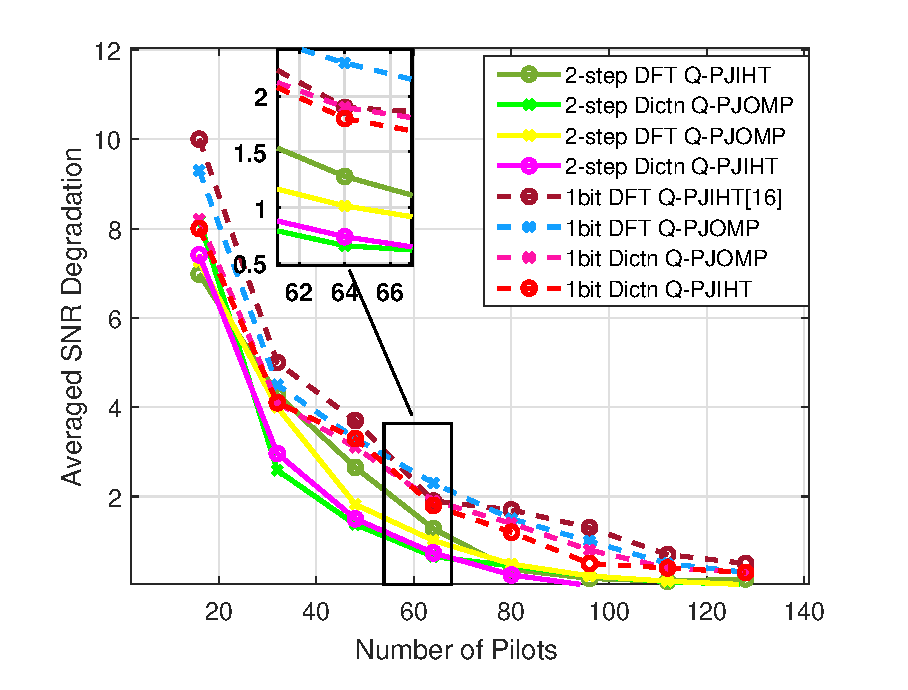
\includegraphics[scale=0.8]{figures/fig_ch_rec/fig2_final.eps}
\caption{Averaged SNR degradation for 1-bit and 2-step quantization using DFT and Dictionary basis  }
\label{Fsnr-deg}
\end{figure}

\begin{figure}[h!]
\centering
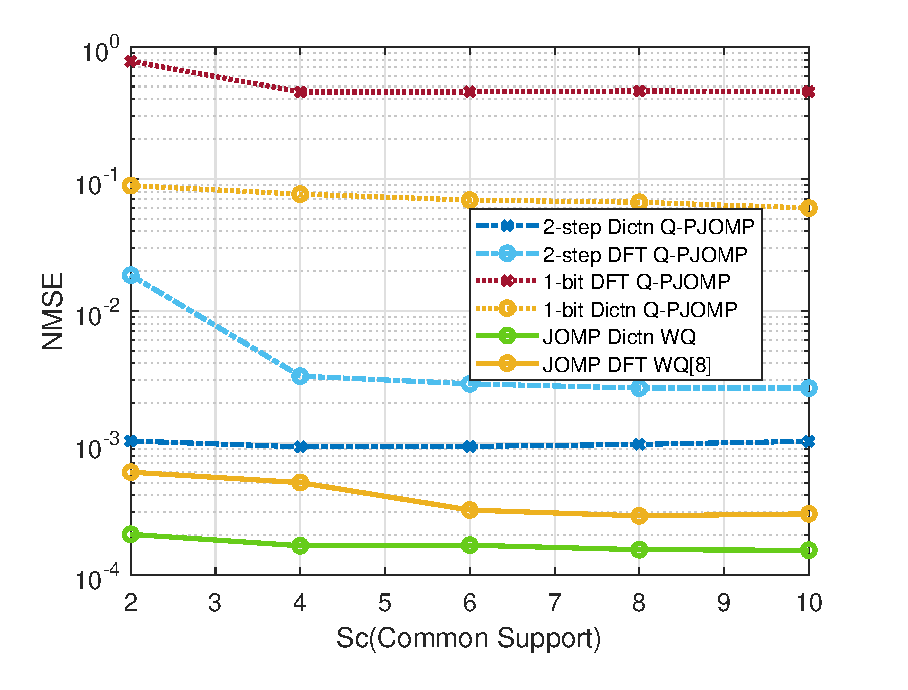
\includegraphics[scale=0.8]{figures/fig_ch_rec/common_support.eps}
\caption{NMSE of CSIT vs common support for 1-bit, 2-step quantization using Q-PJOMP and without quantization(WQ), under P = 45,
$N_t$ = 160, $N_r$ = 2, K = 40, $s_i$ = 17 and transmit SNR = 28 dB.}
\label{sc-jomp}
\end{figure}

\begin{figure}[h!]
    \centering
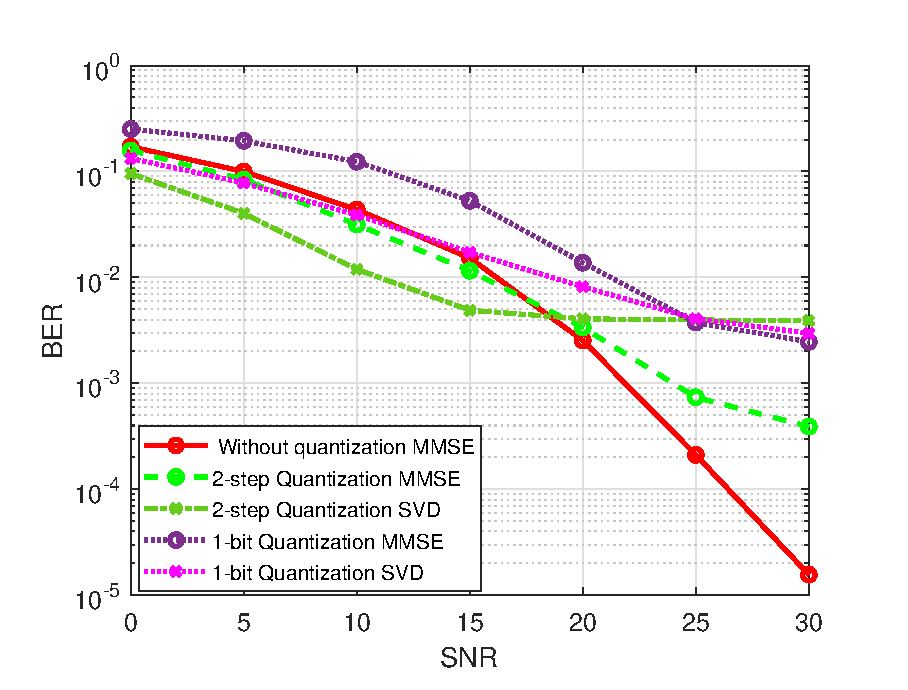
\includegraphics[scale=0.8]{figures/fig_ch_rec/detection-JOMP.eps}
\caption{Averaged Multi-user detection with quantized CSIT based MMSE beamforming (1-bit, 2-step Q-PJOMP) and without quantization (WQ)\label{Fdetection-jomp} } 
\end{figure}
\begin{table} \footnotesize
    \renewcommand{\arraystretch}{1.1}
    \caption{Simulation parameters}
    \label{tabSim}
    \centering
    \begin{tabular}{llr}
        \textbf{Parameter}&\textbf{Symbol}&\textbf{Value}\\
        \hline
        \\
        Transmit antennas & $N_t$&$128$\\
        Receive antennas & $N_r$&$2$\\
        Users            & $K$&$10$\\
        OFDM subcarriers & $N_o$&$256$\\
        OFDM guard interval & $G$&$16$\\
        QAM Modulations & $QAM$&$4$\\
        Multipath channel length & $L$&$6$ \\
        Dictionary length & $M$ & $300$
    \end{tabular}
\end{table}\end{center}

\begin{figure}[h!]
    \centering
    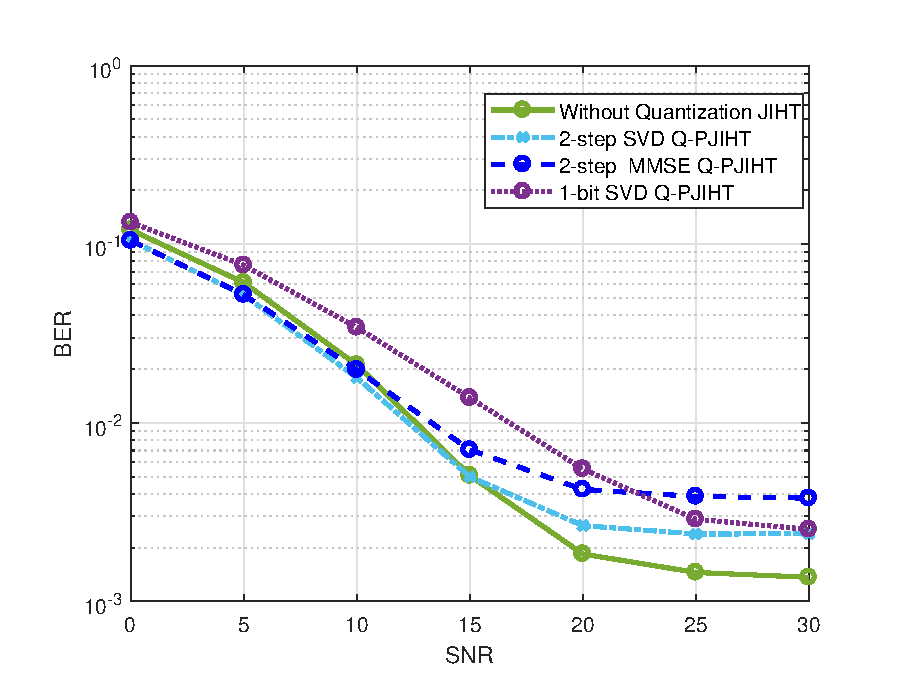
\includegraphics[scale=0.8]{figures/fig_ch_rec/detection_iht.eps}
\caption{Averaged Multi-user data detection with quantized CSIT based beamforming (1-bit, 2-step Q-PJIHT) and without quantization}
\label{Fdetection-JIHT}
\end{figure}

\begin{figure}[h!]
    \centering
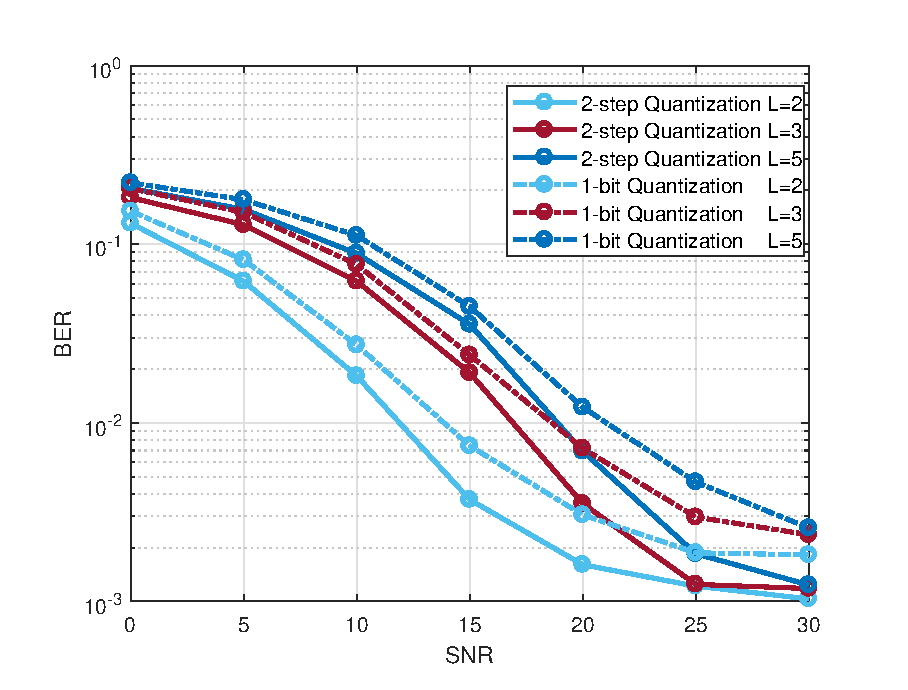
\includegraphics[scale=0.8]{figures/fig_ch_rec/JOMP_L.eps}
\caption{Averaged Multi-user detection with quantized CSIT based beamforming (1-bit, 2-step Q-PJOMP) with varying channel taps $L$ }
\label{Q-PJOMP_L}
\end{figure}
We assume a multipath fading channel with a multipath channel length $L_{taps}$ equal to $6$, whose consequent ISI is directly solved by the OFDM guard interval $G$, moreover, the length of $G$ is set to $16$. The joint sparsity $s_c$ and the individual sparsity $s_i$  parameters are chosen to be  $6$ and  $10$ respectively, where $s_c$ and $s_i$ are defined in Sec. \ref{lbDis_JCS}. 
The summary of the discussion is presented in table \ref{tabSim}, which summarizes the system parameters. In the following subsections, the performance analysis is presented evaluating different metrics, i. e., signal to noise ratio (SNR) degradation, normalized mean squared error (NMSE) as in \cite{mainref-joint}  
for the channel state information at the transmitter (CSIT), and bit error rate (BER) while detecting the data at each user terminal. \\
\subsection{SNR Degradation}
In this subsection, we present the averaged SNR loss obtained using the estimated channel with different numbers of pilot symbols as in \cite{mainref-1bit}. For channel $\mathbf{H}_i$ and its estimate $\mathbf{\hat{H}}_i$, the precoder $\mathbf{w}_i$ is the maximizer of $\|\mathbf{w}_i^H \mathbf{H}_i \mathbf{H}_i^H \mathbf{w}_i\|_2^2$ and $\mathbf{\hat{w}}_i$ is the maximizer of  $\|\mathbf{\hat{w}}_i^H \mathbf{\hat{H}}_i \mathbf{\hat{H}}_i^H \mathbf{\hat{w}}_i\|_2^2$, respectively. The overall SNR loss in $dB$ can be calculated as follows\textcolor{black}{:}
\begin{equation}
    \text{SNR}_{deg}=10\text{log}_{10}\frac{\|\mathbf{w}_i^H \mathbf{H}_i \mathbf{H}_i^H \mathbf{w}_i\|_2^2}{\|\mathbf{\hat{w}}_i^H \mathbf{\hat{H}}_i \mathbf{\hat{H}}_i^H \mathbf{\hat{w}}_i\|_2^2}
    \label{snr_deg}
\end{equation}
Around 200 simulations have been performed to obtain the channel estimate $\mathbf{\hat{H}}_i$ and the precoder $\mathbf{\hat{w}}_i$, which are used in equation (\ref{snr_deg}) to calculate the averaged SNR degradation. Fig. \ref{Fsnr-deg} analyzes the SNR degradation employing Q-PJIHT or Q-PJOMP having 1-bit or  2-step quantization using either DFT or dictionary-based sparsifying matrices. It can be observed that when the feedback overhead approaches $48$ pilots, the SNR degradation exceeds $2$ $dB$ in 1-bit method \cite{mainref-1bit}, which is more than the degradation achieved by the proposed 2 bit Q-PJOMP. Overall, the proposed 2-step Q-PJOMP outperforms the other schemes. 
There are numerous reasons for the better performance of the proposed algorithm: firstly, we have selected a better CS algorithm, i.e., Q-PJOMP, that is more efficient than the IHT based algorithm (Q-PJIHT).   Secondly, since the choice of $\eta$ is critical in IHT \cite{Aiht}, a flexible gradient step size $\eta$ is employed in the Q-PJIHT algorithm. The $\eta$ is used as per sparsity level requirements in each iteration, contrary to a fixed-size of $0.01$  used in \cite{mainref-1bit}.  Thirdly, the 2-step quantization preserves both amplitude and phase information rather than having only direction information as in \cite{mainref-1bit}. Finally, our system employs a dictionary-based sparsifying matrix, which is more robust to estimate the channel as compared to earlier research works \cite{mainref-1bit,mainref-joint}.  This results in better performance with the reduced number of measurements and a fewer number of bits\cite{ourwork}.
Fig. \ref{Fsnr-deg} compares the proposed Q-PJOMP/Q-PJIHT solutions with a 1-bit feedback method  \cite{mainref-1bit}. It can be easily noticed that with $64$ pilots in the magnified view, the proposed quantized feedback  Q-PJOMP with a dictionary-based approach surpasses the performance of almost all feedback based algorithms. Moreover, by increasing the number of pilots, the SNR loss drops down to almost zero for all the solutions. Finally, focusing on the proposed Q-PJOMP method in Fig. \ref{Fsnr-deg}, the 2-step quantization reflects less degradation as compared to the 1-bit quantization.
\subsection{CSIT NMSE analysis Versus common support}
 Fig. \ref{sc-jomp} illustrates the normalized mean square error (NMSE) of CSIT while increasing the common support $s_c$, under the same simulation parameters as in \cite{mainref-joint} for the comparison purpose. The simulation parameters are enlisted as followed: transmit pilot P = 45,
$N_t$ = 160, $N_r$ = 2, K = 40, $s_i = 17$ and transmit $SNR = 28$ dB.
NMSE has been calculated as follows:
\begin{equation}
    \text{NMSE} =\text{E}  \left(\frac{\|\mathbf{H}_i-\mathbf{\hat{H}}_i\|_F}{\|\mathbf{H}_i\|_F} \right)
\end{equation}
The individual and joint sparsity levels are generated using the spatial channel model (SCM)\footnote{3rd generation partnership project(3GPP) and the international telecommunication union(ITU) has developed a spatial channel model(SCM) to model various urban and rural propagation scenarios \cite{SCM}} as in \cite{mainref-1bit,mainref-joint}. Fig. \ref{sc-jomp} reveals as the common support $s_c$ increases among users, the system performance improves, i. e., when the channel between users is more correlated.  These results reinforce our argument that 2-step quantization provides a better estimation than a 1-bit scheme.  It can be observed that the proposed JOMP with a dictionary basis without quantization (WQ) gives better performance than DFT based J-OMP \cite{mainref-joint}.
\subsection{ BER Analysis}
Fig. \ref{Fdetection-jomp} and \ref{Fdetection-JIHT} present the comparison of BER  versus SNR for data detection techniques utilizing SVD and MMSE based beamforming. The channel estimate required for beamforming is obtained using quantized feedback and applying CS techniques such as J-OMP and J-IHT. Moreover, the beamforming obtained without using quantized feedback is presented for comparison purposes.  It is worth noting in Fig. \ref{Fdetection-jomp} that beamforming based on channel estimate obtained using 1-bit feedback and Q-PJOMP has a wider gap as compared to the algorithms without quantization. Moreover, Q-PJOMP with MMSE based precoding gives better results than its SVD counterpart.  \ \
On the contrary, Fig. \ref{Fdetection-JIHT} illustrates that the proposed Q-PJIHT with MMSE precoding performs more inferior as compared to Q-PJIHT with SVD.   By comparing Fig. \ref{Fdetection-jomp} and \ref{Fdetection-JIHT}, it can be observed that Q-PJOMP exhibits better performance as compared to Q-PJIHT, for all the cases with and without quantization. Fig. \ref{Q-PJOMP_L} shows the effect of multipath fading over data detection by employing MMSE beamforming utilizing quantized 1-bit and 2-step feedback using Q-PJOMP based channel estimates.  It can be observed, that as expected by increasing the number of channel taps from $2$ to $5$ the BER performance in all cases is reduces, though the proposed technique yields the improved results.
\subsection{ Computational Complexity Analysis}
Table \ref{tab:comp_time} presents the comparison of computational time per user for 2-step and 1-bit Q-PJOMP/Q-PJIHT. Three different transmit antennas setting has been considered: $N_t=[50, 100, 150]$. 
As expected, the computational time increases with the number of transmit antennas. Furthermore, the 2-step algorithms (Q-PJOMP/Q-PJIHT) are more expensive than 1-bit methods. This is due to the processing of the channel amplitude information, and rebuilding complex pilots from both amplitude and direction information, nevertheless, the analysis reveals that the difference is not very significant. 
Finally, comparing Q-PJOMP with Q-PJIHT, iterative hard thresholding based algorithms are generally much slower than the orthogonal matching pursuit based techniques, since they require a certain number of iteration to reach an optimal point.   
\begin{table}[h!]
    \caption{ COMPUTATION COMPLEXITY COMPARISON FOR MU-MASSIVE MIMO UNDER PARAMETRIC SETTING  P = 45, N = 2, K = 40, $s_c$ = 9, $s_i$ = 17, P = 28 dB AND $N_t$= 50,100, 180. }
\label{tab:comp_time}
\centering
%\addtolength{\tabcolsep}{-2pt}
 \begin{tabular}{||c |c |c |c ||} 
 \hline
Time(s)&$N_t$=50&$N_t$=100&$N_t$=150\\ [0.9ex] 
 \hline\hline
 2-step Q-PJOMP&$1.2 \times10^{-3}$&$1.4 \times10^{-3}$ & $1.6 \times10^{-3}$ \\ [0.9ex]
 \hline
 1-bit Q-PJOMP& $9.24\times10{-4}$&$1.2 \times10^{-3}$& $1.3\times10^{-3}$ \\[0.9ex]
 \hline
 2-step Q-PJIHT& $6.86\times10^{-2 }$& $7.19\times10^{-2 }$&$7.38\times10^{-2 }$  \\[0.9ex]
 \hline
 1-bit Q-PJIHT&$5.82\times10^{-2 }$& $6.94\times10^{-2 }$&$7.02\times10^{-2 }$ \\[1ex] 
 \hline
\end{tabular}
\end{table}

\section{Conclusion}
We have presented distributed compressed sensing based channel estimation techniques for the partially joint channel in a massive MIMO system.  Especially, a novel Q-PJOMP and Q-PJIHT based channel estimation algorithms utilizing limited quantized feedback are proposed. The proposed system reduces training and feedback overhead by employing a fewer number of pilots along with a limited number of feedback bits for channel estimation. Moreover, the channel is jointly recovered for all users by applying DCS at BS from 2-step quantized feedback. \\
The results revealed that SNR degradation with 2-step quantized feedback is less than 1 dB for 64 pilots. Furthermore, as the number of pilots grows, the SNR degradation approaches closer to zero. Additionally, the presented dictionary-based system aids in reducing the training and feedback overhead. This is achieved by exploiting an improved CS  algorithm and pilot design. Finally, when the channel among users is highly correlated and exhibits added common support, the jointly estimated channel at BS will reduce the computational resources and time. The future work comprises of extending the proposed massive MIMO scheme to localization issues for improving performance  \cite{LocalizationICC2013,LocalizationTVT2016}, this could be achieved by exploiting a large number of serving antennas.
